% Drawing 70/03-6 -- folder 70, batch 03, archive page 59 (PDF page 60).
% Transcription: page de figures seules, reprenant celle de la p.~52 : en haut, un digone hachuré (deux arêtes joignant deux sommets) et un triangle à trois sommets marqués ; à droite, le sommet $s_0$ avec les arêtes $a_0$ (vers $s_1$), $a_1$ (vers $s_2$), $a_2$ (vers $s_3$) et les faces $f_0$, $f_1$ ; au centre, la figure développée : de $s_0$ partent $a_0$ vers $s_1$, $a_1$ vers $s_2$, $a_2$ vers $s_3$ et une quatrième arête vers le bas ; faces $f_0$ (hachurée, entre $a_0$ et $a_1$), $f_1$ (entre $a_2$ et $a_0$), $f_2$ (sous $a_1$), $f_3$ au-delà de $s_1$, et en $s_1$ l'arête $a_2'$. Le reste de la page est blanc.
% Kind: page of figures: digon, triangle, vertex stars. Method 2 (schematic redraw from the facsimile). Status: ok.
% Notes: Top left: a digon (two arcs joining two points) hatched under its upper arc, and a triangle with two marked vertices and a doubled top stroke. Top right: the star of s_0: a line through s_0 carrying a_0 (thick, to s_1, then continued), a_2 up to s_3, a_1 (thick) to s_2 (continued beyond it), labels f_1, f_0 and hatching between a_0 and a_1. Centre, the developed figure: from s_0 the edges a_2 (arrow, up to s_3), a_0 to s_1, a_1 to s_2 and a fourth edge down (arrow); from s_1 an edge up (with a short branch) and a'_2 down to the right; faces f_1, f_0, f_2, f_3; hatching as short strokes near s_0 (between a_2 and a_0, under a_0, under a_1) and along a'_2. All edges at a vertex start exactly at it. Left out: an ink blot left of the centre figure and some faint pencil strokes above s_1. Nothing is struck. The rest of the page is blank. Redrawn 2026-11-09 (issue 128) after Michel's check: vertices placed once and every edge drawn between them, so concurrent lines meet exactly; labels at \small. 2026-11-13, Claude Opus 5.5, overlay check (issue 147): laid over the scan rendered at 350 dpi in colour, whole and zoomed (20-50 px a unit); not compiled (no TeX engine in the session), the TikZ was rasterised by a script. The edges, vertices, labels and the two small figures at the top lie on their ink within about 1 unit (the edges kept meeting exactly at their vertices, as asked on 9 November). Corrected: the hatching of the centre figure near s_0, re-read at 50 px a unit: between a_2 and a_0 it is five faint strokes slanting down to the right (they were drawn slanting the other way), and under a_0 five strokes hanging from the edge (they were drawn across it); the long stroke reaching a_0 above f_0 is the ascender of the f and is not hatching. Left out as before: the ink blot, the faint pencil strokes above s_1, and also the faint arrow-like marks scattered over the page (set-off) and the small mark before s_0.
% Coordinates: 1 unit = 1 mm = 1/100 of the crop width (bbox in page fractions: [0.1, 0.06, 0.62, 0.34]).
% Redrawn by Claude (claude-opus-5-5), issue #73, 2026-11-09; not checked by a human; not compiled (no TeX in the session).
% Rights: reproduces part of the work -- behind RENDER_TRANSCRIPTS, never published by itself.
\documentclass[tikz,border=3pt]{standalone}
\usepackage{amsmath,amssymb}
\usetikzlibrary{patterns,arrows.meta}
\tikzset{pencil/.style={black!45}, struck/.style={black!35}, mark/.style={circle,draw,inner sep=1.3pt}, pt/.style={circle,fill,inner sep=0.9pt}, opt/.style={circle,draw,fill=white,inner sep=1.1pt}}
\begin{document}
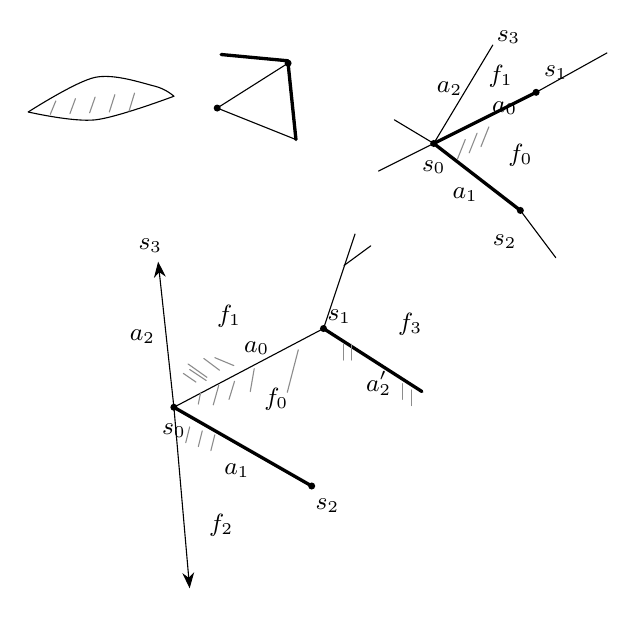
\begin{tikzpicture}[x=1mm,y=1mm,line cap=round,line join=round,font=\scriptsize]
\draw plot[smooth, tension=0.55] coordinates {(21.5,-13) (30,-8.6) (37.5,-9.7) (40,-11)};
\draw plot[smooth, tension=0.55] coordinates {(21.5,-13) (30,-14) (40,-11)};
\draw[pencil] (25,-11.6) -- (24.3,-13.3);
\draw[pencil] (27.5,-11.3) -- (26.8,-13.2);
\draw[pencil] (30,-11.1) -- (29.3,-13.1);
\draw[pencil] (32.5,-10.8) -- (31.8,-13);
\draw[pencil] (35,-10.6) -- (34.3,-12.9);
\draw (45.5,-12.5) -- (54.5,-6.8);
\draw[very thick] (54.5,-6.8) -- (55.5,-16.5);
\draw (45.5,-12.5) -- (55.5,-16.5);
\draw[very thick] (46,-5.7) -- (54.5,-6.5);
\node[pt] at (45.5,-12.5) {};
\node[pt] at (54.5,-6.8) {};
\draw (66,-20.5) -- (73,-17);
\draw[very thick] (73,-17) -- (86,-10.5);
\draw (86,-10.5) -- (95,-5.5);
\draw (73,-17) -- (80.5,-4.5);
\draw[very thick] (73,-17) -- (84,-25.5);
\draw (84,-25.5) -- (88.5,-31.5);
\draw (68,-14) -- (73,-17);
\node[pt] at (73,-17) {};
\node[pt] at (86,-10.5) {};
\node[pt] at (84,-25.5) {};
\draw[pencil] (76,-19) -- (77,-16.5);
\draw[pencil] (77.5,-18.2) -- (78.5,-15.7);
\draw[pencil] (79,-17.4) -- (80,-14.9);
\node[inner sep=1pt] at (82.5,-3.5) {\small $s_3$};
\node[inner sep=1pt] at (75,-10) {\small $a_2$};
\node[inner sep=1pt] at (81.5,-8.5) {\small $f_1$};
\node[inner sep=1pt] at (88.5,-8) {\small $s_1$};
\node[inner sep=1pt] at (82,-12.5) {\small $a_0$};
\node[inner sep=1pt] at (73,-20) {\small $s_0$};
\node[inner sep=1pt] at (84,-18.5) {\small $f_0$};
\node[inner sep=1pt] at (77,-23.5) {\small $a_1$};
\node[inner sep=1pt] at (82,-29.5) {\small $s_2$};
\draw[-{Stealth[length=2mm]}] (40,-50.5) -- (38,-32);
\draw (40,-50.5) -- (59,-40.5);
\draw[very thick] (40,-50.5) -- (57.5,-60.5);
\draw[-{Stealth[length=2mm]}] (40,-50.5) -- (42,-73.5);
\draw (59,-40.5) -- (63,-28.5);
\draw (61.6,-32.5) -- (65,-30);
\draw[very thick] (59,-40.5) -- (71.5,-48.5);
\node[pt] at (40,-50.5) {};
\node[pt] at (59,-40.5) {};
\node[pt] at (57.5,-60.5) {};
\draw[pencil] (41.8,-45) -- (44.2,-46.7);
\draw[pencil] (42,-45.7) -- (44.1,-47.1);
\draw[pencil] (41.2,-46.2) -- (42.8,-47.3);
\draw[pencil] (43.8,-44.3) -- (45.8,-45.8);
\draw[pencil] (45.2,-44.2) -- (47.6,-45.2);
\draw[pencil] (43.4,-48.6) -- (43.1,-50.1);
\draw[pencil] (45.7,-47.7) -- (45,-50.2);
\draw[pencil] (47.7,-47.2) -- (47,-49.5);
\draw[pencil] (50.2,-45.6) -- (49.7,-48.5);
\draw[pencil] (55.8,-43.2) -- (54.4,-48.6);
\draw[pencil] (42,-53) -- (41.5,-55);
\draw[pencil] (43.6,-53.5) -- (43.1,-55.5);
\draw[pencil] (45.2,-54) -- (44.7,-56);
\draw[pencil] (61.5,-42.5) -- (61.5,-44.5);
\draw[pencil] (62.5,-42.5) -- (62.5,-44.5);
\draw[pencil] (69,-47.5) -- (69,-49.5);
\draw[pencil] (70.2,-48.3) -- (70.2,-50.3);
\node[inner sep=1pt] at (37,-30) {\small $s_3$};
\node[inner sep=1pt] at (36,-41.5) {\small $a_2$};
\node[inner sep=1pt] at (47,-39) {\small $f_1$};
\node[inner sep=1pt] at (50.5,-43) {\small $a_0$};
\node[inner sep=1pt] at (61,-39) {\small $s_1$};
\node[inner sep=1pt] at (70,-40) {\small $f_3$};
\node[inner sep=1pt] at (53,-49.5) {\small $f_0$};
\node[inner sep=1pt] at (66,-47.5) {\small $a'_2$};
\node[inner sep=1pt] at (40,-53.5) {\small $s_0$};
\node[inner sep=1pt] at (48,-58.5) {\small $a_1$};
\node[inner sep=1pt] at (59.5,-63) {\small $s_2$};
\node[inner sep=1pt] at (46,-65.5) {\small $f_2$};
\end{tikzpicture}
\end{document}
